\subsection{The rotation periods of cool main-sequence stars}

The \citet{mcquillan2014} catalog was the first large-scale stellar rotation
period catalog, generated from analyzing light curves from the \kepler\
spacecraft and remains one of the most valuable community products in the
field of stellar astronomy.
It contains around 34,000 rotation periods of FGKM dwarfs and subgiants,
measured from autocorrelation functions (ACFs) of light curves.
This catalog revealed a gap in the rotation periods of K and M dwarfs: a strip
in the rotation vs effective temperature plane that is under-populated
compared to the surrounding parts of parameter space.
This gap can be seen in figure \ref{fig:the_gap}.
\begin{figure}
  \caption{
The rotation periods of 18,259 FGKM dwarf stars, measured by \mct, vs. their
effective temperatures.
We applied cuts to the \gaia\ color-magnitude diagram of these stars (figure
\ref{fig:CMD_cuts}) in order to remove equal-mass binaries and subgiants from
the sample.
The rotation period gap can be seen as an almost-horizontal gap toward the
right of this figure.
}
  \centering
    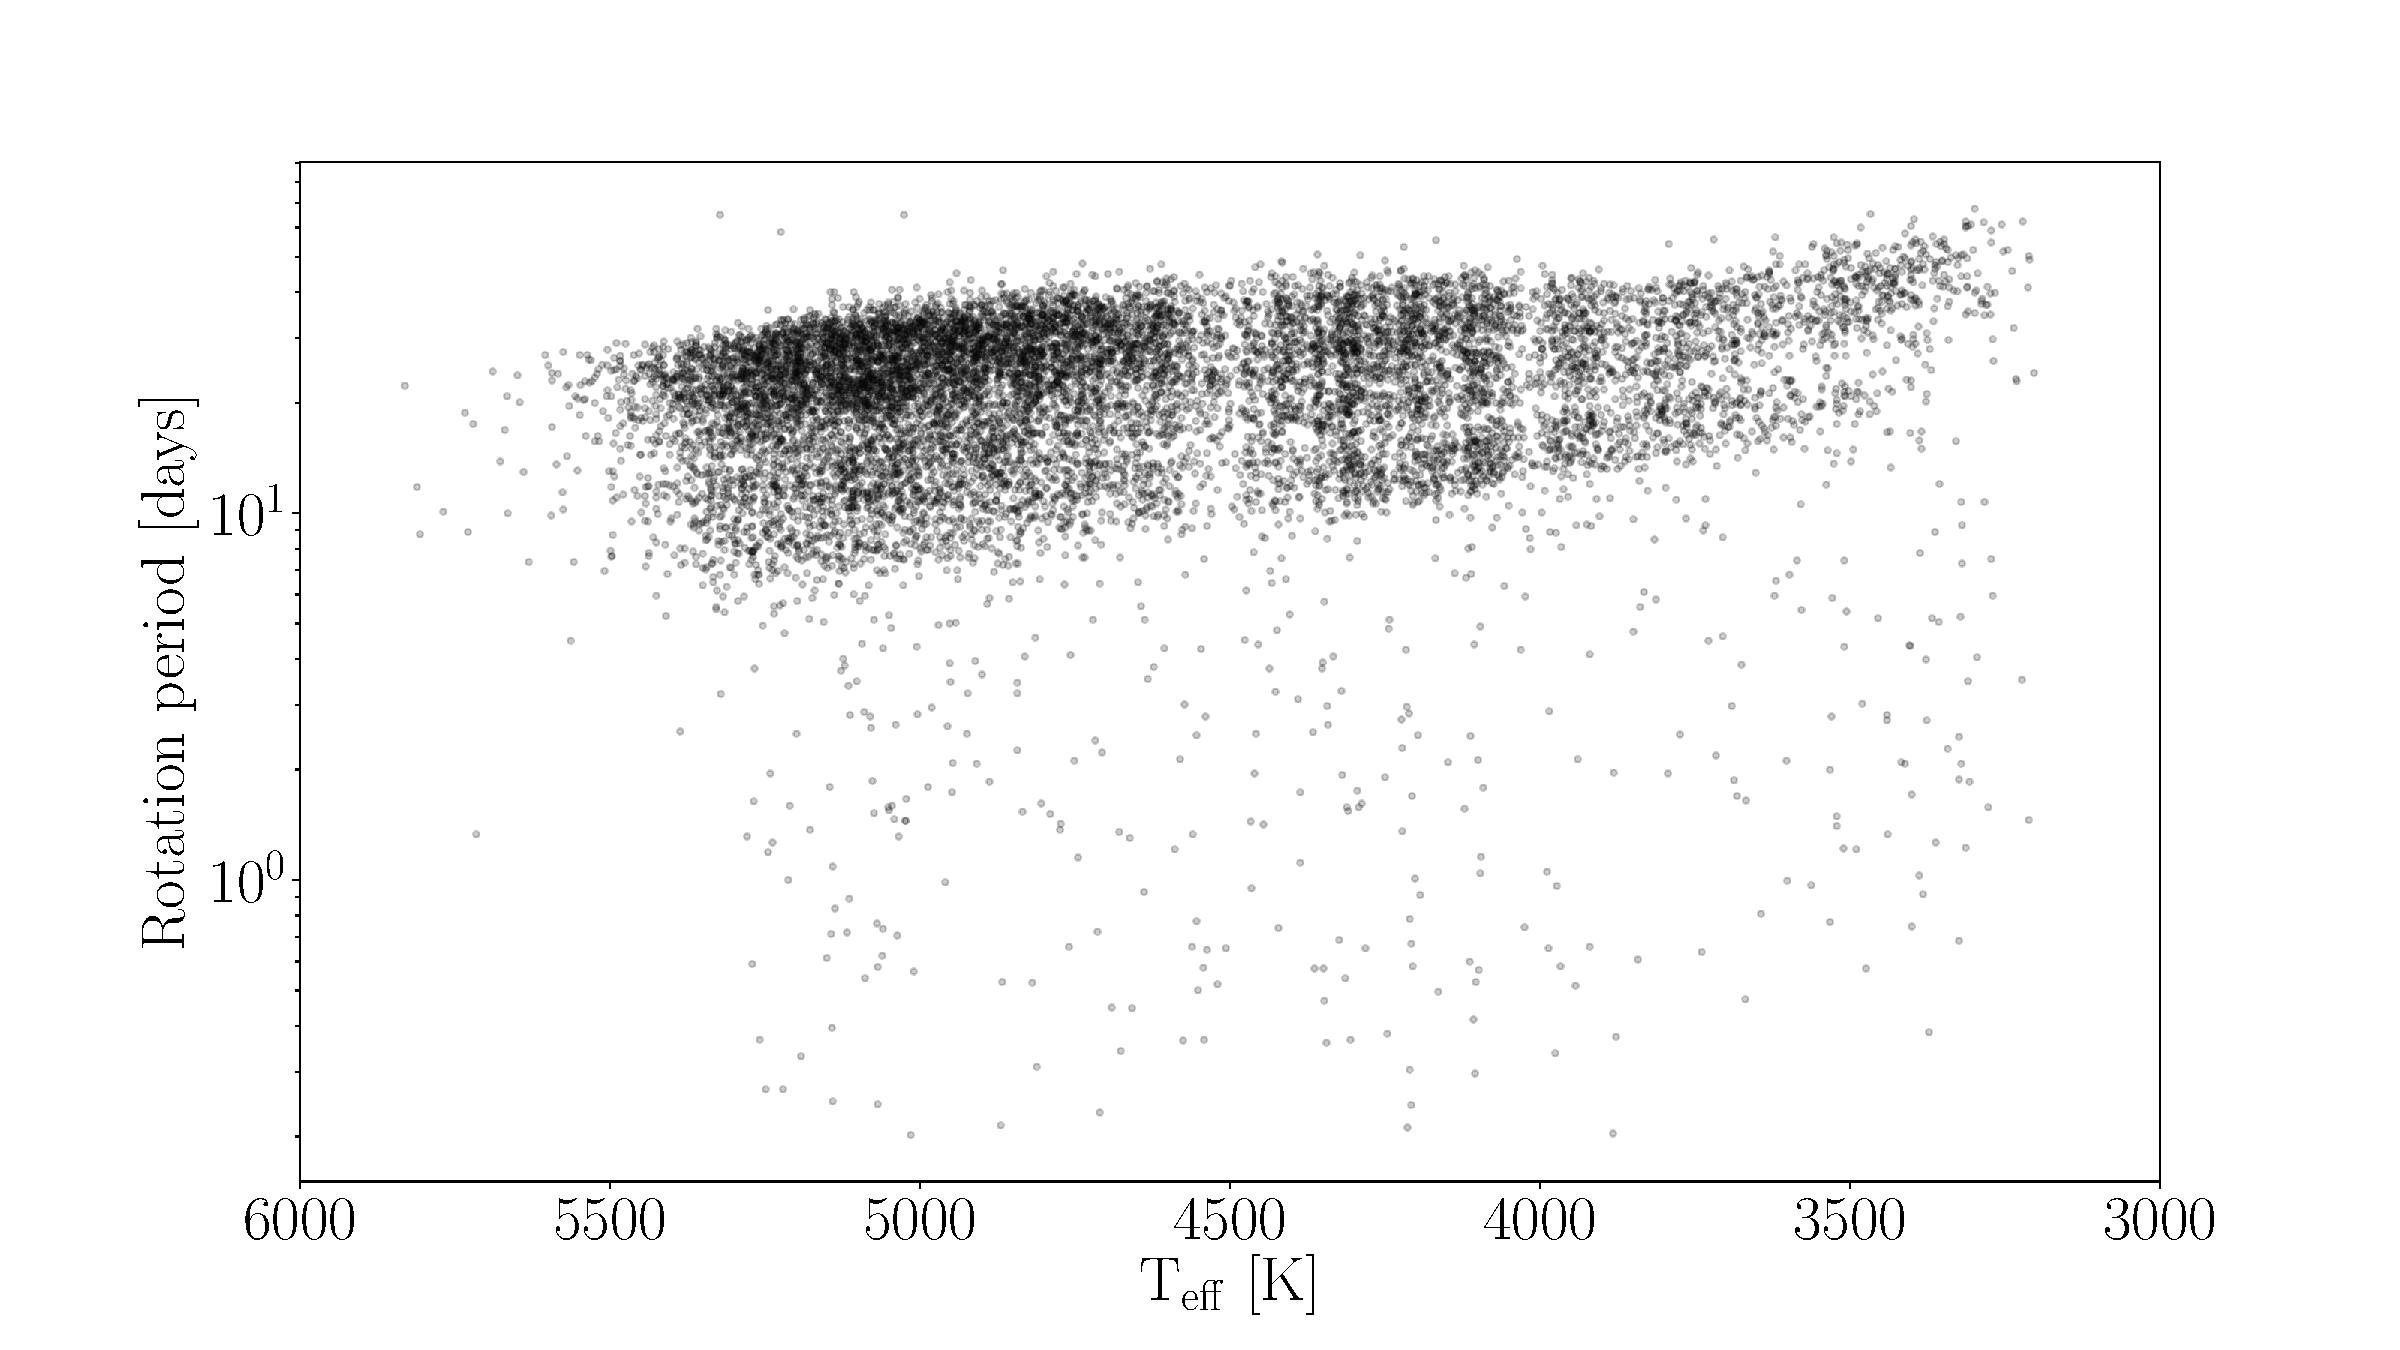
\includegraphics[width=1\textwidth]{the_gap}
\label{fig:the_gap}
\end{figure}
The rotation period gap is most prevalent for low-mass stars, of spectral type
K and M, but was recently shown to extend through G, F and A types as well
\citep{davenport2017}.

Three explanations for the origin of this gap have been proposed.
Firstly, since the gap falls on what is thought to be an isochrone in
period-effective temperature space, it follows that it may be caused by a
discontinuity in the age distribution of the sample.
The gap could be created if there exist two populations of stars with
different age distributions, with the distribution of young ages peaking at
around 800 Myr, and the distribution of old ages peaking at around 2-3 billion
years.
This idea was investigated by \mct, who suggested that the two populations
might be the thin and thick disk of the Milky Way.
However, they found no sharp change in kinematic properties between the two
samples.
In addition, the thin/thick disk transition is thought to be around 6-8 Gyr,
which is older than the majority of stars in the \mct\ sample
\racomment{(citations)}.
A short pause in star formation is difficult to explain by invoking, \eg\ the
passage of a spiral arm through the Solar neighbourhood, since an increase in
gas density would be expect to boost, not quench, star formation rate.
However perhaps the Solar neighbourhood passed between two spiral arms around
1 billion years ago, however pattern speed, orbital period (200 Myrs)... seems
unlikely.
Possible passage of a dwarf galaxy but, again, this would be expected to boost
star formation, not suppress it.

The second explanation for the rotation period gap is that stars either
transition rapidly across the gap, \ie\ experience a rapid phase of angular
momentum loss at an age of around 1 billion years, or become magnetically
inactive for a short period of time such that their rotation periods become
undetectable.
This first scenario could be caused by a sudden recoupling between the core
and envelope, where core and envelope rotate differentially before the gap,
then angular momentum is radially redistributed and stars rotate as solid
bodies after the gap.
The latter scenario is hinted at by \citet{reinhold2017} who noticed that the
amplitudes of light curves decrease smoothly either side of the gap, as though
stars gradually become more inactive until they have no large-scale surface
features and their rotation periods become almost impossible to detect.
\citet{reinhold2017} suggest that a transition between a spot-dominated and
faculae-dominated regime could lead to a cancelling-out of surface features.
% do not lose
% angular momentum uniformly over time: instead they undergo a period of rapid
% spin down at an age of around 1.1 Gyr, or a Rossby number of around...
% \racomment{(Calculate this!)}.
% Since the rotation period gap is located along a line of constant Rossby
% number \racomment{(what is this number?)}, and since the rate of stellar
% angular momentum loss is known to be related to magnetic field strength , it
% follows that the gap could be caused by some phenomenon related to magnetic
% braking.
% (this
% is the principle behind gyrochronology \citep[\eg][]{kawaler1989,
% pinsonneault1989, barnes2003, barnes2007, angus2015, vansaders2016,
% vansaders2018, angus2019})

The final explanation for the rotation period gap is one of measurement error
or confounding by binarity.

As of May 2019, the \citet{mcquillan2014} catalog has been used more than 250
times, for a range of studies spanning fields from exoplanets to white dwarfs,
to galactic archaeology.
Since it underpins so many astronomical studies, a large number of incorrectly
measured rotation periods in this catalog would undermine several of the
studies built upon it.

\subsection{Using kinematics to solve the mystery}

Stars are thought to be born in the thin disk of the Milky Way, orbiting the
center of the galaxy with a low out-of-plane, or vertical, velocity ($W$, or
$v_z$).
Young stars have relatively small vertical velocities, but gain momentum in
the vertical direction over time.
Although the cause of orbital heating is not well understood, interactions
with giant molecular clouds and spiral arms are thought to play an important
role \racomment{(citations)}.
Although the velocity of any individual star will only provide a weak age
constraint, the velocity dispersion of a group of stars can indicate whether,
on average, that group is old or young relative to other groups.
In this work we compare the velocity dispersions of groups of stars to
ascertain which groups are older and which younger and draw conclusions based
on the implied relative ages of populations.
% Stellar velocities have a history of being used as an age proxy, with several
% notable examples within stellar astronomy \citep[\eg][]{faherty2009,
% west2011}.
Since the age-velocity dispersion relations (AVRs) are themselves still
actively being calibrated, it is difficult to directly compare gyrochronal
ages with kinematic ones.
However, regardless of the exact relation between velocity dispersion and
stellar age, it is expected to be a monotonic relationship, therefore velocity
dispersion can be used effectively to {\it rank} groups of stars by age.

% Vertical {\it actions} are better age indicators than velocities, because
% actions are calculated by integrating angular momentum over the Milky Way's
% potential, and are therefore position invariant -- \eg\ a star will have the
% same action at periapsis and apoapsis.
% In contrast, orbital velocities are different at periapsis and apoapsis -- so
% in this sense, {\it actions} are the natural quantities to use as age proxies.
Vertical action is a better age indicator than vertical velocity, however both
vertical action ($J_z$) and vertical velocity (\vz/W) can only be calculated
with full 6-dimensional position and velocity information.
Unfortunately, most stars with measured rotation periods do not have radial
velocity (RV) measurements because they are relatively faint \kepler\ targets
($\sim$11th-18th magnitudes).
For this reason, we used an alternative age proxy: velocity in the direction
of galactic latitude, \vb.
The \kepler\ field is positioned at low galactic latitude (b=5-20\degrees), so
\vb\ is a close approximation to \vz.

% The rotation periods of middle-aged FGKM stars are mostly determined by their
% mass, age and evolutionary stage, and this is due, for the most part, to
% angular momentum loss through magnetic braking.
% Although stars are born with a range of rotation periods, a steep dependence
% of angular momentum loss, $J$ angular frequency, $\omega$, $J \propto
% \omega^3$ causes stellar rotation periods to converge after a characteristic
% timescale.
% This timescale is on the order of a few tens of millions of years for F and G
% stars, but hundreds of millions of years for K and M stars.
% Once stars exceed this age, they steadily lose angular momentum via magnetized
% stellar winds that remove angular momentum from the star at a radius that is
% determined by the magnetic field strength.
% The Rossby number, the ratio of rotation period to convective turnover
% timescale, is linked to the strength of stellar magnetic dynamos.
% Large-scale polodial and toroidal stellar magnetic fields are thought to be
% generated by the $\alpha-\Omega$ mechanism, whereby convective motion of
% plasma and differential stellar rotation cause the winding up of magnetic
% field lines, generating a strong magnetic field \racomment{(citations)}.
% In general, the ratio between a star's rotation period and its characteristic
% timescale of convective motion (the Rossby number) determines the strength of
% the magnetic field \racomment{(citation)}.
% Stars that rotate quickly and have deep convection zones, therefore long
% convective turnover times, have small Rossby numbers and strong magnetic
% fields.
% Young M dwarfs typically have the strongest magnetic fields.
% Slowly rotating stars with shallow convective zones, such as old F and G
% dwarfs, have weak magnetic fields \racomment{(citations)}.
% Since magnetic field strength depends on stellar rotation period and mass via
% the Rossby number, it follows that angular momentum loss driven by magnetized
% stellar winds also depends on Rossby number.
